% tex file for clustering 
\par The main part of our analysis comes from different 
implementations of procedures for multiple comparisons between the subjects.
More specifically, we focused on an implementation of the Benjamini-Hochberg 
procedure, the grouping of t-statistics, and the grouping of $\hat{\beta}$ 
values. We also explored clustering with hierarchical clustering. We found 
appropriate parameters to be used for all subjects by observing the images 
from a few subjects at different 
points of input for each of the three analyses. The parameters that we played 
around with include the false discovery rate, the cutoff value for significant 
t-values and $\hat{\beta}$-values, and the number of neighbors that we wanted 
smooth the data over in the analysis. For hierarchical clustering using the 
ward metric, we compared different parameter selections of number of clusters.

\subsubsection{Benjamini-Hochberg Correction}

\par When conducting multiple comparisons, it is important to have an 
idea of the quantity of Type I errors that may be prevalent in the analysis. 
In our analysis of voxel data, we decided that limiting/controlling the number 
of Type I errors is important to the process. The processes of limiting the 
number of Type I errors are called FDR-controlling procedures. In the grand 
scheme of things, FDR-controlling procedures give greater statistical power 
with the cost of more Type I errors that can fall through. 

\par Once we implemented the hypothesis function that would return t-test 
values and ``p-values'', we implemented the Benjamini-Hochberg procedure to 
control the proportion of rejected null hypotheses in the data. The Benjamini-
Hochberg procedure works by multiplying each of the ``p-values'' to a ratio of 
the number of tests times the rank of the ``p-value'' in the ordered set, 
and the chosen false discovery rate -- from these adjusted 
``p-values'', only the values that are less than the chosen false discovery 
rate will be chosen to be returned. This way, we are able to adjust the 
proportion of null hypotheses that will be rejected and the proportion that 
will return the desired proportion of significant tests. This will reduce the
number of false positives returned in the data and extend greater statistical 
power in later analysis performed on the voxel dataset.

\par The Benjamini-Hochberg procedure was not the only analysis we did over the
multiple subjects. After completing t-grouping with t-statistics, and value 
grouping with $\hat{\beta}$ values, we noticed that the variability between the
subjects of the study is different between the Benjamini-Hochberg procedure 
outputs, and the t-statistics and $\hat{\beta}$ value grouping procedure 
outputs. Moreover, when performing the Benjamini-Hochberg procedure, along with
the t-statistics grouping procedures, we did play around with smoothing over 
neighboring voxels. Ultimately, however, we decided to forgo the neighbor 
smoothing to prevent loss of information in the plots that we generated in the 
end, and neighbor smoothing didn't visually appear very needed.



\subsubsection{t-Statistics Grouping}

\par We use the t-statistics that we found earlier for another type of cutoff
analysis. The t-statistics measure the size of the difference relative to the 
variation in the data. Thus, a small ``p-value'' corresponds directly to large
absolute values of t-statistics. In fact, the ``p-value'' and the t-statistics
are related by the following statement: More extreme t-statistics will return 
lower ``p-values'', which increases the chances of the null hypothesis being 
indicated as false. Although the t-statistics go hand in hand with the 
Benjamini-Hochberg analysis on the ``p-values'', we ultimately decided that an 
additional process of selecting t-statistics based on a threshold was 
necessary because the ``p-values'' assume a normal distribution while the 
t-statistics do not assume this from the data. It should be noted that the 
t-statistics grouping analysis performed as well, if not better, than the 
``p-value'' analysis using the Benjamini-Hochberg procedure.

\par Since the magnitude from zero represents how significant the test is for
t-statistics, we collected the absolute value t-statistics that were above a 
certain threshold. This was the opposite of the procedure for finding the 
significant tests in the Benjamini-Hochberg process. The threshold, also called
the cutoff in the scripts that were written when developing this process, is 
calculated in a very similar fashion to the Benjamini-Hochberg false discovery 
rate. This is because the t-values and the ``p-values'' are strongly linked, in 
fact there is a 1-to-1 relation between the absolute value of t - values to 
p-values.

\par Implementing the t-value grouping function was almost trivial because it 
is the flip side of the Benjamini-Hochberg function that was implemented 
previously. However, since we do not know if there's a function that relates 
the absolute values of t-statistics to ``p-values'', there was a lot of 
experimenting with different values to see which values of cutoff points versus
false discovery rates (the Q value in the Benjamini-Hochberg function) would 
deliver similarly focused results.

\subsubsection{$\hat{\beta}$ Grouping}

\par Using the same function that we created to group a certain subset of the 
t-statistics, we also looked over the $\hat{\beta}$ values as a part of our 
analysis. Much of what we know in statistics tells us that observing 
$\hat{\beta}$ values on top of looking at t-statistics would not tell us much 
since the two variables are not explicitly connected; however, the main reason 
why we decided it was of utmost importance to look at both the t-statistics 
and the $\hat{\beta}$ values is that there might be a relationship between the 
trends in each respective variables' output to the cutoff point, that is lost
when going from $\hat{beta}$ to t-statistic (dividing by variance). 

\par Granted, it is pretty clear that the t-statistics grouping is very 
theoretically similar to the Benjamini-Hochberg procedure. This is why the 
$\hat{\beta}$ grouping portion of the analysis was added on. Since $\hat{\beta}$ 
values do not directly use normality assumptions, we thought it would offer 
either a different angle on how to approach analysis, or confirm the results 
found in the analysis that depended on the assumptions of normality. 

\subsubsection{Hierarchical Clustering}

\par Using the across-subject average t-statistics for every voxel in the
brain, we are left with a 3-d array of t-statistics that contain both negative
and positive values. Instead of manually observing patterns in these images, we
instead implemented a clustering algorithm to split the entire 3-d images into
clusters based on the voxels' relative location to each other as well as the
values of their t-statistics.

\par In order to find a proper clustering algorithm, we decided to treat this
problem like a grayscale image segmentation problem and implemented a
agglomerative hierarchical cluster using Ward's method. Agglomerative means
that the clusters are built bottom up with each observation starting as its
own cluster and pairs being moved up the hierarchy. Ward's method creates
clusters based on a minimum variance criterion that minimizes the total
within-cluster variances. An example of this implementation for a 2-d image is
seen here: 
\url{http://scikit-learn.org/stable/auto_examples/cluster/plot_lena_ward_segmen
tation.html}.

In our implementation, we defined a structure to our data using a connectivity
graph in order to ensure that each cluster is spatially constrained. Also,
since our scenario uses a 3-d image, the connectivity graph will also have to
take into account this extra dimension.

\par Ultimately, we did not use this clustering algorithm in our main paper
because it did not add any useful information on top of our other clustering
methods we used. See figure \ref{fig:cluster_comparison} to see similarities. 
Furthermore, we faced a few
problems when trying to implement the algorithm. Most significantly, creating
the 3-d connectivity graph was a problem, and we were not able to properly
implement this in z-direction. Furthermore, runtime was an issue when compared
to our other options. Ultimately, the idea around using a hierarchical
clustering method was intriguing; however, the same results could be achieved
using simpler and faster methods.


\subsubsection{Comparison of Clustering Techniques}
Generally the clustering techniques for the multiple comparison and the 
hierarchical clustering produces similar results, which can be seen if a 
side by side comparison of the hierarchical clustering method using Ward
against the quantile-based clustering algorithm for t-statistics (we've
included the actual t-values as well in the center for comparisons) 
[Figure \ref{fig:cluster_comparison}]. Depending upon the subject, the clustering 
from Benjamini Hochberg, t grouping and $\hat{\beta}$ grouping can be 
very different or very similar.



% Put in an image for playing around with parameters (Ben?)
\begin{figure}[ht]

	\centering
	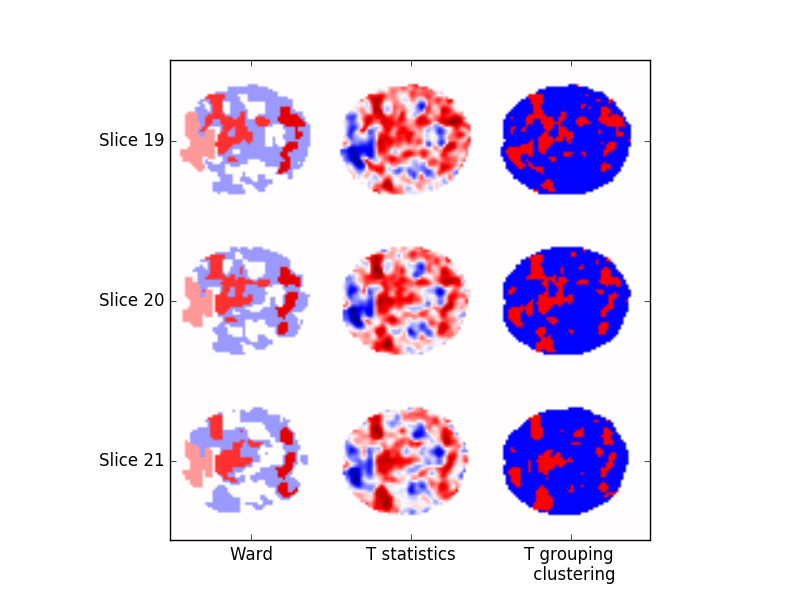
\includegraphics[width=.8\linewidth]{../images/cluster_comparison.png} 
	\caption{Clustering Comparison between WARD, t-statistics, and t-grouping}
	\label{fig:cluster_comparison}

\end{figure}
